%%%%%%%%%%%%%%%%%%%%%%%%%%%%%%%%%%%%%%%%%%%%%%%%%%%%%%%%%%%%%%%%%%%
%%%%%%%%%%%%%%%%%%%%%%%%%%%%%%%%%%%%%%%%%%%%%%%%%%%%%%%%%%%%%%%%%%%
%\begin{frame}{Problems with integration in Deep Learning}
%\begin{center}
%We have to fix a quadrature rule 
%
%without information about the trial space.
%
%\vspace{0.7cm}
%
%\arrowdown
%
%\vspace{0.7cm}
%
%If we use fix quadrature points, the solution may be erroneous.
%\end{center}
%
%\end{frame}
%%%%%%%%%%%%%%%%%%%%%%%%%%%%%%%%%%%%%%%%%%%%%%%%%%%%%%%%%%%%%%%%%%%
\begin{frame}{Challenge 2: The need for Quadrature Rules}

\begin{tikzpicture}
\node  at (7,0.0){
\begin{tikzpicture}
\begin{axis}[scale only axis, xlabel = $\textcolor{white}{E}x\textcolor{white}{E}$, ylabel = $u$, ytick pos=left, y label style={at={(-0.1,0.5)}},  legend style= {at={(0.6,0.98)},draw=none,fill=none,nodes={scale=0.8, transform shape}}, legend cell align={left}, height=3.5cm,title= Exact and approximate solutions, xticklabel style={yshift=-2pt},]

% \end{figure}idth=4cm, xmin=-0.2, ymin=0, xmax=10.2, ymax=50]
\addlegendimage{only marks, mark=-, color=black} 
\addlegendimage{only marks, mark=-, color=red}
\addplot [black, line width=0.7pt,domain=0:10] {x^0.7};
%\addlegendentry{Exact solution}
\addplot[line width=0.5pt,color=red] %
	table[x=x ,y=u_pred]{frames/Javi/data/data_Ritz_normal.csv};
%\addlegendentry{Gauss/AD};

% Legend
\node[anchor = south] (Ua)at (6,32){\textcolor{red}{$u_{NN}$}};
\node[anchor = south] at (6,4){\textcolor{black}{$u_{exact = x^{0.7}}$}};
\end{axis}
\end{tikzpicture}
};

%

\node at (0,0.05){
\begin{tikzpicture}
\begin{axis}[scale only axis, xlabel = $Epoch$, ylabel = $Loss$, ytick pos=left, y label style={at={(-0.05,0.7)}}, legend style= {at={(0.85,0.4)},draw=none,fill=none,nodes={scale=0.8, transform shape}}, legend cell align={left}, height=3.5cm, width=6cm, xmin=0.95, ymin=-15, xmax=45000, ymax=12, ytick = {8,-1.538,-15}, xmode=log, title = $\mathcal{L}_{Ritz}$ evolution,]
\addplot [red, dashed, line width=0.7pt,domain=0.99999:39900] {-1.538};

\addplot[line width=0.8pt,color=black] %
	table[x=epoch ,y=loss]{frames/Javi/data/loss_Ritz_normal_treshold.csv};
\node at (140, -3.2){\textcolor{red}{$Loss \; expected \;(minimum \;energy) $}};
\node at (40, 3.){$Loss \; computed$};
\end{axis}
\end{tikzpicture}
};

%%%%%%%Problem
\node [anchor = west] at (-2, 4) {
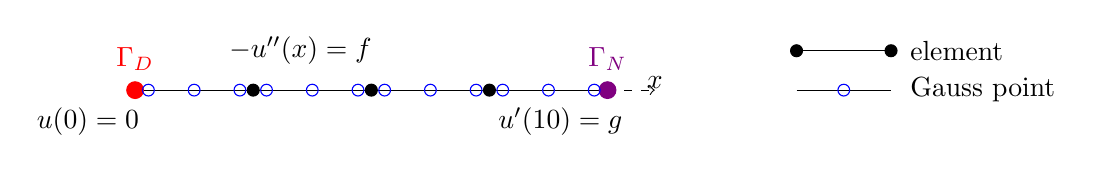
\begin{tikzpicture}[x=0.6cm, y=1cm]
\draw[-] (0,0) -- (10,0);
\draw[->, dashed] (10,0) -- (11,0);
%
\draw[red,fill=red] (0,0) circle (0.7ex);
\draw[violet,fill=violet] (10,0) circle (0.7ex);
\node [red] at (0,0.4){$\Gamma_D$};
\node [violet] at (10,0.4){$\Gamma_N$};
\node at (3.5,0.5){$-u''(x) = f $};
\node at (-1,-0.4){$u(0) = 0$};
\node at (9.,-0.4){$u'(10) = g$};
\node at (11,0.1){$x$};

\draw[black,fill=black] (2.5,0) circle (0.5ex);
\draw[black,fill=black] (5,0) circle (0.5ex);
\draw[black,fill=black] (7.5,0) circle (0.5ex);

\node [draw, circle, blue ,  inner sep=-1.5] (G1K1) at (0.28175, 0){};
\node [draw, circle, blue ,  inner sep=-1.5] (G2K1) at (1.25, 0)   {};
\node [draw, circle, blue ,  inner sep=-1.5] (G3K1) at (2.21825, 0){};

\node [draw, circle, blue ,  inner sep=-1.5] (G1K2) at (2.5+0.28175, 0){};
\node [draw, circle, blue ,  inner sep=-1.5] (G2K2) at (2.5+1.25, 0)   {};
\node [draw, circle, blue ,  inner sep=-1.5] (G3K2) at (2.5+2.21825, 0){};

\node [draw, circle, blue ,  inner sep=-1.5] (G1K3) at (5+0.28175, 0){};
\node [draw, circle, blue ,  inner sep=-1.5] (G2K3) at (5+1.25, 0)   {};
\node [draw, circle, blue ,  inner sep=-1.5] (G3K3) at (5+2.21825, 0){};

\node [draw, circle, blue ,  inner sep=-1.5] (G1K4) at (7.5+0.28175, 0){};
\node [draw, circle, blue ,  inner sep=-1.5] (G2K4) at (7.5+1.25, 0)   {};
\node [draw, circle, blue ,  inner sep=-1.5] (G3K4) at (7.5+2.21825, 0){};

%\node at (7,0.2){4 elements with};
\draw[-] (14,0.5) -- (16,0.5);
\draw[black,fill=black] (14,0.5) circle (0.5ex);
\draw[black,fill=black] (16,0.5) circle (0.5ex);
\node [anchor =west] at (16.2,0.5){element};

\draw[-] (14,0.) -- (16,0.);
\node [draw, circle, blue ,  inner sep=-1.5] (G3K4) at (15, 0){};
\node [anchor =west] at (16.2,0.){Gauss point};
\end{tikzpicture}
};

\end{tikzpicture}
\end{frame}
%%%%%%%%%%%%%%%%%%%%%%%%%%%%%%%%%%%%%%%%%%%%%%%%%%%%%%%%%%%%%%%%%%%

%%%%%%%%%%%%%%%%%%%%%%%%%%%%%%%%%%%%%%%%%%%%%%%%%%%%%%%%%%%%%%%%%%%
\begin{frame}{Challenge 2: The Need for Quadrature Rules}
\begin{tikzpicture}
\node at (7,0){
\begin{tikzpicture}
\begin{axis}[scale only axis, xlabel = $\textcolor{white}{Ep}x\textcolor{white}{Ep}$, ylabel = $u_{NN}$, ytick pos=left, y label style={at={(0,0.5)}}, height=4cm, width=4cm, xmin=0, ymin=18, xmax=2.5, ymax=50, ticks=none,
title = Solution in one element,]
%\addlegendimage{only marks, mark=-, color=black} 
%\addlegendimage{only marks, mark=-, color=red}
%\addplot [black, line width=0.7pt,domain=0:10] {x^0.7};
%\addlegendentry{Exact solution}
\addplot[line width=0.5pt,color=red] %
	table[x=x ,y=u_pred]{frames/Javi/data/data_Ritz_normal.csv};
\addplot[only marks, blue, mark size=2, mark=o] coordinates {
      (0.28175, 19)
      (1.25, 46.27)
      (2.21825, 36.05)
    };
%
\node(G)[anchor = north, text width=1.0] at (axis cs: 1.5,30)
 {\textcolor{blue}{Gauss points}};
\node(G_aux1)[anchor = north, text width=1.0] at (axis cs: 1.65,31) {};
\node(G_aux2)[anchor = north, text width=1.0] at (axis cs: 2,31) {};
    

\node (G1) at (axis cs: 0.28175, 19){};
\node (G2) at (axis cs: 1.25, 46.27){};
\node (G3) at (axis cs: 2.21825, 36.05){};

\draw[] (G1) node[above, blue] {};
\draw[] (G2) node[above, blue] {};
\draw[] (G3) node[above, blue] {};


\path[->, blue] (G) edge (G1);
\path[->, blue] (G_aux1) edge (G2);
\path[->, blue] (G_aux2) edge (G3);
\end{axis}
\end{tikzpicture}
};

\node at (0,0){
\begin{tikzpicture}
\begin{axis}[scale only axis, xlabel = $Epoch$, ylabel = $Loss$, ytick pos=left,  legend style= {at={(0.85,0.4)},draw=none,fill=none,nodes={scale=0.7, transform shape}}, legend cell align={left}, height=4cm, width=6cm, xmin=0.95, ymin=-15, xmax=45000, ymax=12, 
ticks=none, 
%title style={at={(0.5,0)},anchor=north,yshift=-0.1},
title = $\mathcal{L}_{Ritz}$ evolution,
 xmode=log]
\addplot [red, dashed, line width=0.7pt,domain=0.99999:39900] {-1.538};
%\addlegendentry{$F_R(u)$ (Loss of the exact solution)};
\addplot[line width=0.8pt,color=black] %
	table[x=epoch ,y=loss]{frames/Javi/data/loss_Ritz_normal_treshold.csv};
%\addlegendentry{$F_R(u_{NN})$ (Loss of the approximation)};
\node at (140, -3.2){\textcolor{red}{$Loss \; expected \;(minimum \;energy) $}};
\node at (40, 3.){$Loss \; computed$};
\end{axis}
\end{tikzpicture}
};
\end{tikzpicture}

\vspace{-0.3cm}
$$
\notag
\mathcal{L}_{Ritz} (u_{NN}) \approx \frac{1}{2} \sum_{i=1}^{Nq} \omega_i\, \textcolor{red}{\underbrace{\textcolor{black}{\left( \nabla u_{NN}(x_{i}) \right)^2}}_{\rightarrow 0}}
 - \sum_{i=1}^{Nq} \omega_i\, f(x_{i}) \,  \textcolor{red} {\underbrace{\textcolor{black}{{u_{NN}(x_{i})}}}_{\rightarrow \infty}} -g(x\big|_{\Gamma_N}) \, u_{NN}(x\big|_{\Gamma_N}).
$$

\end{frame}